%%%%%%%%%%%%%%%%%%%%%%%%%%%%% Define Article %%%%%%%%%%%%%%%%%%%%%%%%%%%%%%%%%%
\documentclass{article}
%%%%%%%%%%%%%%%%%%%%%%%%%%%%%%%%%%%%%%%%%%%%%%%%%%%%%%%%%%%%%%%%%%%%%%%%%%%%%%%

%%%%%%%%%%%%%%%%%%%%%%%%%%%%% Using Packages %%%%%%%%%%%%%%%%%%%%%%%%%%%%%%%%%%
\usepackage{geometry}
\usepackage{graphicx}
\usepackage{amssymb}
\usepackage{amsmath}
\usepackage{amsthm}
\usepackage{empheq}
\usepackage{mdframed}
\usepackage{booktabs}
\usepackage{lipsum}
\usepackage{graphicx}
\usepackage{color}
\usepackage{psfrag}
\usepackage{pgfplots}
\usepackage{bm}
%%%%%%%%%%%%%%%%%%%%%%%%%%%%%%%%%%%%%%%%%%%%%%%%%%%%%%%%%%%%%%%%%%%%%%%%%%%%%%%

% Other Settings

%%%%%%%%%%%%%%%%%%%%%%%%%% Page Setting %%%%%%%%%%%%%%%%%%%%%%%%%%%%%%%%%%%%%%%
\geometry{a4paper}

%%%%%%%%%%%%%%%%%%%%%%%%%% Define some useful colors %%%%%%%%%%%%%%%%%%%%%%%%%%
\definecolor{ocre}{RGB}{243,102,25}
\definecolor{mygray}{RGB}{243,243,244}
\definecolor{deepGreen}{RGB}{26,111,0}
\definecolor{shallowGreen}{RGB}{235,255,255}
\definecolor{deepBlue}{RGB}{61,124,222}
\definecolor{shallowBlue}{RGB}{235,249,255}
%%%%%%%%%%%%%%%%%%%%%%%%%%%%%%%%%%%%%%%%%%%%%%%%%%%%%%%%%%%%%%%%%%%%%%%%%%%%%%%

%%%%%%%%%%%%%%%%%%%%%%%%%% Define an orangebox command %%%%%%%%%%%%%%%%%%%%%%%%
\newcommand\orangebox[1]{\fcolorbox{ocre}{mygray}{\hspace{1em}#1\hspace{1em}}}
%%%%%%%%%%%%%%%%%%%%%%%%%%%%%%%%%%%%%%%%%%%%%%%%%%%%%%%%%%%%%%%%%%%%%%%%%%%%%%%

%%%%%%%%%%%%%%%%%%%%%%%%%%%% English Environments %%%%%%%%%%%%%%%%%%%%%%%%%%%%%
\newtheoremstyle{mytheoremstyle}{3pt}{3pt}{\normalfont}{0cm}{\rmfamily\bfseries}{}{1em}{{\color{black}\thmname{#1}~\thmnumber{#2}}\thmnote{\,--\,#3}}
\newtheoremstyle{myproblemstyle}{3pt}{3pt}{\normalfont}{0cm}{\rmfamily\bfseries}{}{1em}{{\color{black}\thmname{#1}~\thmnumber{#2}}\thmnote{\,--\,#3}}
\theoremstyle{mytheoremstyle}
\newmdtheoremenv[linewidth=1pt,backgroundcolor=shallowGreen,linecolor=deepGreen,leftmargin=0pt,innerleftmargin=20pt,innerrightmargin=20pt,]{theorem}{Theorem}[section]
\theoremstyle{mytheoremstyle}
\newmdtheoremenv[linewidth=1pt,backgroundcolor=shallowBlue,linecolor=deepBlue,leftmargin=0pt,innerleftmargin=20pt,innerrightmargin=20pt,]{definition}{Definition}[section]
\theoremstyle{myproblemstyle}
\newmdtheoremenv[linecolor=black,leftmargin=0pt,innerleftmargin=10pt,innerrightmargin=10pt,]{problem}{Problem}[section]
%%%%%%%%%%%%%%%%%%%%%%%%%%%%%%%%%%%%%%%%%%%%%%%%%%%%%%%%%%%%%%%%%%%%%%%%%%%%%%%

%%%%%%%%%%%%%%%%%%%%%%%%%%%%%%% Plotting Settings %%%%%%%%%%%%%%%%%%%%%%%%%%%%%
\usepgfplotslibrary{colorbrewer}
\pgfplotsset{width=8cm,compat=1.9}
%%%%%%%%%%%%%%%%%%%%%%%%%%%%%%%%%%%%%%%%%%%%%%%%%%%%%%%%%%%%%%%%%%%%%%%%%%%%%%%

%%%%%%%%%%%%%%%%%%%%%%%%%%%%%%% Title & Author %%%%%%%%%%%%%%%%%%%%%%%%%%%%%%%%
\title{Unidad 3 - AMN 2024}
\author{Rodrigo Miranda}
%%%%%%%%%%%%%%%%%%%%%%%%%%%%%%%%%%%%%%%%%%%%%%%%%%%%%%%%%%%%%%%%%%%%%%%%%%%%%%%

\begin{document}
    \maketitle
\section{Extrapolacion de Richardson}
\subsection{Ejemplo 1}
Emplee la extrapolacion de Richardson para aproximar $g'(-0.65)$mediante $ N_6(h)$, si:
\\ \indent \indent $g(x)=xlog(x+2)-x^2cos^{-1}(e^{2x})$
\noindent \\Use un $h=1/100$. Ademas, obtenga el valor exacto y el error en la aproximacion. Emplee 15 decimales.  

\noindent \\ \textbf{Nota:} Cuando nos dicen que usaremos un $N_6(h)$, significa que usaremos una matriz cuadrada de orden 6. (6 columnas, 6 filas.)

\begin{figure}[ht]
    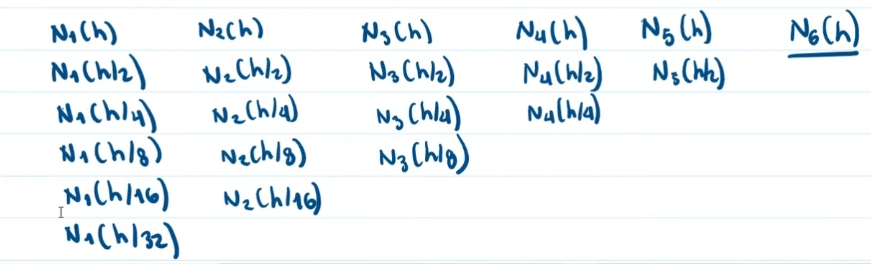
\includegraphics[scale=0.6]{img/eje1_1.png}
\end{figure}
\noindent \\ El siguiente paso, es meter la funcion g(x) que nos dan, en Matlab
\\ $>> syms x\\
>> g = x*log10(x + 2) - x^2*acos(exp(2*x));\\
>> c=-0.65;\\
>> h=1/100;\\
>> N=zeros(6)\\$
\\ \textbf{Donde: }g, es la ecuacion que nos dan. c, es el valor g' que nos dan. y N, la matriz llena de 0, de 6x6 que nos pide el ejercicio.
\\ \begin{theorem}[Formula centrada de 3 puntos.]
    $f'(c)=\frac{f(c+h)-f(c-h)}{2h}$
\end{theorem}
\noindent \\ Ahora, debemo ir llenando la matriz de acuerdo a su posicion y la formula aplicada en dicha posicion.
\\ $N(1,1)=(subs(g,c+h)-subs(g,c-h))/(2*h);$




\section{Newton- Cotes}
\subsection{Ejemplo 1}

\noindent \\ Determine el volumen del solido generadp al rotar alrededor de la recta $y=5$, la region acotada
por las graficas de $y=x^2,y=4x-x^2$ empleando las formulas de Newton-Cotes con n=5 y n=6.
Ademas, obtenga el valor exacto y el error de la aproximacion. Emplee 15 decimales,
\begin{figure}[ht]
    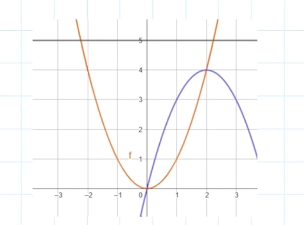
\includegraphics[scale=0.6]{img/nc1_1.png}  
\end{figure}
\\ \textbf{Formula cerrada de Newton-Cotes con n=5}
\\ Que estamos viendo? Bueno, en lo primero que nos vamos a fijar es en la region encerrada por las dos graficas
Luego, imaginaremos que esa seccion esta girando en el eje y=5. Por la forma de la grafica, debemos trabajar con el metodo de arandelas.
\begin{figure}[ht]
    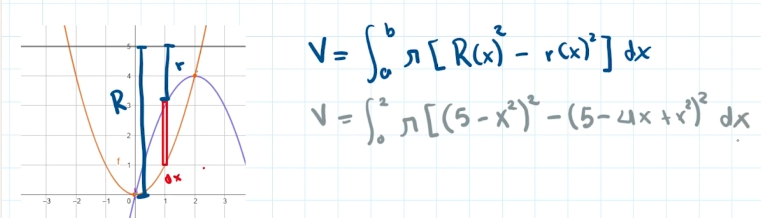
\includegraphics[scale=0.8]{img/nc1_2.png}  
\end{figure}
\\ Como sacamos el planteamiento? Bueno, R, sera representada por la grafica concaba haci arriba, mientra r sera representada por la grafica concaba hacia abajo.
Posterior a esto, debemo analizar el eje de rotacion, observamos que el eje es y=5 y dado que el metodo de arendales nos hace trazar 
nuestro dx de forma perpendicular, podemos analizar que nuestra R estara determinada por el eje de rotacion (5) - la funcion del radio externo. Mientras que r
sera determinada por 5 - la fumcion del radio interno.
\begin{figure}[ht]
    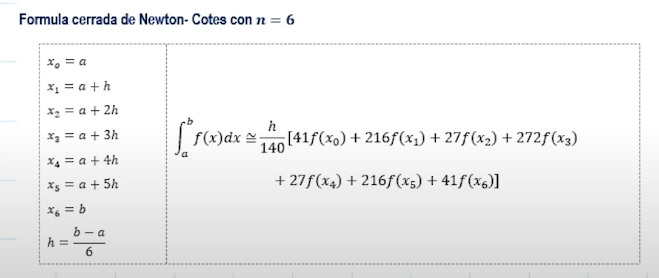
\includegraphics[scale=0.8]{img/nc1_3.png}  
\end{figure}
\begin{theorem}[Formula cerrada de Newton-Cotes con n=6]
    $\int_{a}^{b} f(x) \,dx \cong \frac{h}{140}[41f(x0)+216f(x1)+27f(x2)+272f(x3)+27f(x4)+216f(x5)+41f(x6)]$
\end{theorem}



\end{document}